\documentclass[conference,a4paper]{IEEEtran}

% Author-year citations as in the supervisor's examples: [Mnih et al. 2015] and Mnih et al. [2015].
% For round brackets, as in the AAAI-style examples, replace "square" with "round".
\usepackage[square,authoryear]{natbib}
\setcitestyle{aysep={}}
\renewcommand{\bibfont}{\footnotesize}
\setlength{\bibsep}{2pt}
\usepackage{amsmath,amssymb}
\usepackage{graphicx}
\usepackage{booktabs}
\usepackage{array}
\usepackage{tikz}
\usetikzlibrary{positioning,arrows.meta}
\usepackage{url}
\usepackage[hidelinks]{hyperref}

\graphicspath{{../analysis_output/corrected-rct-01/report/}{figures/}}
\newcommand{\results}{../analysis_output/corrected-rct-01/report}

\begin{document}

\title{INVESTIGATING DEEP Q-LEARNING
MODIFICATIONS WITH RANDOMISED
CONTROL TRIALS}

\author{\IEEEauthorblockN{Matimu Khosa}
\IEEEauthorblockA{\textit{School of Computer Science and Applied Mathematics}\\
\textit{University of the Witwatersrand}\\
Johannesburg, South Africa\\
2716924@students.wits.ac.za\\[3pt]
Supervised by Steven James and Benjamin Rosman}}

\maketitle

\begin{abstract}
Extensions to the deep Q-network (DQN) are usually evaluated with their own tuned hyperparameters and a handful of
random seeds, so a reported gain may reflect the configuration rather than the extension. We evaluate four
extensions, namely Double DQN, prioritised experience replay (PER), multi-step returns and Averaged DQN, in a paired
randomised control trial. Thirty hyperparameter configurations were sampled from a shared population, each with
its own seed, and every configuration was trained with DQN and with each extension on four MinAtar games, giving
600 runs of five million frames. The primary outcome was the area under the greedy evaluation curve, compared with
DQN by paired t-tests with a Bonferroni correction across all sixteen comparisons. Averaged DQN improved on DQN in
Asterix, Freeway and Space Invaders, by 57.5, 20.9 and 19.5 per cent in mean AUC. Double DQN improved only in Space
Invaders, by 11.4 per cent. PER was worse in Freeway and Space Invaders, and multi-step returns were
worse in Asterix, Freeway and Space Invaders, by up to 80 per cent. No extension differed detectably from DQN in
Breakout. On the scale of per-configuration AUC ratios, seven of these nine findings remained significant; the gains
of Averaged DQN in Asterix and of Double DQN in Space Invaders did not. Final-checkpoint endpoints agreed in direction
with all nine findings but detected fewer of them, trials of three to ten configurations often missed them, and
comparing the best configuration of each method reversed two of them. Under a shared training recipe, Averaged DQN
was the only extension that improved on DQN in more than one game.
\end{abstract}

\begin{IEEEkeywords}
deep reinforcement learning, deep Q-network, experimental design, randomised control trial, MinAtar, sample
efficiency
\end{IEEEkeywords}

% =====================================================================================
\section{Introduction}

The deep Q-network (DQN) of \citet{mnih2015human} learnt to play Atari 2600 games from pixels, using two
stabilising devices: experience replay and a periodically updated target network. Many extensions followed, each
changing one part of the algorithm. Double DQN changes how the bootstrap target is computed \citep{vanhasselt2016deep},
prioritised experience replay (PER) changes which transitions are replayed \citep{schaul2016prioritized}, multi-step
($n$-step) returns lengthen the horizon of the target \citep{hernandezgarcia2019understanding,sutton2018reinforcement},
and Averaged DQN averages the estimates of several earlier target networks \citep{anschel2017averaged}. Rainbow
combined several such components and, in an ablation, found prioritised replay and multi-step learning to be the two
most important \citep{hessel2018rainbow}.

Each extension was, however, introduced with its own training recipe and evaluated on its own configuration. Deep
reinforcement learning results are sensitive to hyperparameters, random seeds and implementation
details \citep{henderson2018deep}, evaluation protocols differ between papers \citep{machado2018revisiting}, and
comparisons often rest on few runs and point estimates \citep{colas2018many,agarwal2021deep}. When an extension
outperforms DQN under one tuned configuration, it is therefore hard to say whether the gain belongs to the
extension or to the configuration.

We address this with a randomised control trial in the sense of \citet{pretorius2020dropout}. The
individuals of the trial are hyperparameter configurations sampled from a shared population, and every individual
receives every treatment. Each comparison with DQN is then paired on the same configuration and seed, which removes
the main effect of the configuration from the comparison while still averaging over the population. We use the
MinAtar suite \citep{young2019minatar}, whose small observations make 600 full training runs feasible on CPUs.

We ask two research questions. \emph{RQ1:} across a population of configurations and under one shared training
recipe, does each extension change sample efficiency, measured as the area under the evaluation curve (AUC),
relative to DQN? \emph{RQ2:} how far can the conclusions of smaller or more typical evaluations, based on a single
checkpoint, a few configurations or the best configuration of each method, be trusted relative to those of the full
trial? Our contributions are:
\begin{itemize}
\item a paired trial of four DQN extensions on 30 sampled configurations and four MinAtar games (600 runs,
$3\times10^{9}$ frames), with code, raw results and provenance released\footnote{\url{https://github.com/2716924/research_project}};
\item evidence that, under the shared recipe, Averaged DQN is the only extension that improves on DQN in more than one
game, that the benefit of Double DQN is small and fragile, and that PER and $n$-step returns are harmful;
\item evidence that effects vary across the population: the learning rate changes the AUC by as much as the largest
treatment effects, and in Freeway the $n$-step deficit is concentrated at the rate every other arm prefers;
\item evidence that single-checkpoint endpoints and small trials lack power, and that comparing the best configuration
of each method can reverse a conclusion.
\end{itemize}
Section~\ref{sec:background} reviews background and related work, Section~\ref{sec:method} describes the trial,
Section~\ref{sec:results} reports the results, Section~\ref{sec:discussion} discusses them and
Section~\ref{sec:limitations} states the limitations.

% =====================================================================================
\section{Background and Related Work}\label{sec:background}

\subsection{Deep Q-Networks}
\begin{figure}[t]
\centering
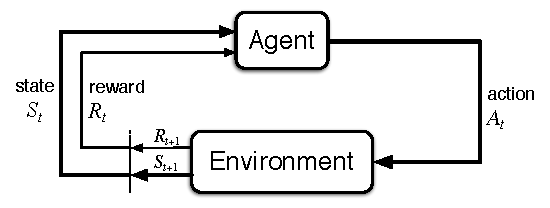
\includegraphics[width=\columnwidth]{agent_environment.pdf}
\caption{The agent--environment interaction in a Markov decision process. Reproduced from
\citet{sutton2018reinforcement}.}
\label{fig:agent_env}
\end{figure}

An agent interacting with a Markov decision process observes a state $s_t$, takes an action $a_t$, receives a
reward $r_{t+1}$ and moves to $s_{t+1}$; it seeks to maximise the expected return discounted by
$\gamma\in[0,1)$ \citep{sutton2018reinforcement} (Fig.~\ref{fig:agent_env}). Q-learning \citep{watkins1992q} estimates the optimal action-value
function by bootstrapping from $\max_{a'}Q(s',a')$. DQN \citep{mnih2015human} approximates $Q$ with a neural network
with parameters $\theta$, stores transitions in a replay buffer $\mathcal{D}$ \citep{lin1992self} and minimises
\begin{equation}
L(\theta)=\mathbb{E}_{(s,a,r,s')\sim U(\mathcal{D})}\big[(y-Q(s,a;\theta))^2\big]
\label{eq:loss}
\end{equation}
with the target
\begin{equation}
y=r+\gamma\max_{a'}Q(s',a';\theta^-),
\label{eq:dqn}
\end{equation}
where $\theta^-$ are the parameters of a target network copied from $\theta$ every $C$ steps, and $y=r$ when $s'$
is terminal.

\subsection{The Four Extensions}\label{sec:extensions}
\emph{Double DQN} \citep{vanhasselt2016deep}. The maximum in~\eqref{eq:dqn} uses the same estimates to select and
to evaluate the next action, which biases the target upwards. Double DQN selects the action with the online network
and evaluates it with the target network:
\begin{equation}
y=r+\gamma\,Q\big(s',\textstyle\arg\max_{a'}Q(s',a';\theta);\theta^-\big).
\end{equation}

\emph{Prioritised experience replay} \citep{schaul2016prioritized}. Instead of sampling uniformly, PER samples
transition $i$ with probability
\begin{equation}
P(i)=\frac{p_i^{\alpha}}{\sum_k p_k^{\alpha}},\qquad p_i=|\delta_i|+\epsilon,
\end{equation}
where $\delta_i$ is the latest temporal-difference (TD) error of the transition. New transitions receive the largest
priority seen so far. Importance-sampling weights $w_i=(|\mathcal{D}|\,P(i))^{-\beta}/\max_j w_j$ correct the bias
of non-uniform sampling, with $\beta$ annealed linearly to 1. For the proportional variant used here,
\citet{schaul2016prioritized} chose $\alpha=0.6$ and $\beta_0=0.4$ by a coarse grid search on eight games, with Double
DQN rather than DQN as the base agent, and they reduced the step size by a factor of four relative to that agent because
prioritised replay picks high-error transitions more often, which makes the typical gradient larger.

\emph{Multi-step returns} \citep{hernandezgarcia2019understanding,sutton2018reinforcement}. The $n$-step target sums
$n$ observed rewards before bootstrapping:
\begin{equation}
y=\sum_{k=0}^{n-1}\gamma^k r_{t+k+1}+\gamma^n\max_{a'}Q(s_{t+n},a';\theta^-).
\end{equation}
Without an off-policy correction, as in Rainbow \citep{hessel2018rainbow}, the reward sum follows the exploratory
behaviour policy rather than the greedy policy, which trades bias for faster propagation of reward.

\emph{Averaged DQN} \citep{anschel2017averaged}. Averaged DQN keeps the last $K$ target networks
$\theta^-_1,\dots,\theta^-_K$ and averages their action values before taking the maximum:
\begin{equation}
y=r+\gamma\max_{a'}\frac{1}{K}\sum_{k=1}^{K}Q(s',a';\theta^-_k).
\label{eq:avg}
\end{equation}
This reduces the variance of the target approximation error at the cost of $K$ forward passes per target, with the
same number of gradient updates as DQN \citep{anschel2017averaged}.

\subsection{Component Studies}
Rainbow's ablation on 57 Atari games found that removing prioritised replay or multi-step learning caused the
largest drops in median performance \citep{hessel2018rainbow}. \citet{obandoceron2021revisiting} repeated the
additive and ablative studies on smaller environments, including the five MinAtar games, and found multi-step returns
to be the component that most improved DQN on MinAtar. Their agents used the Adam optimiser \citep{kingma2015adam}
and fixed hyperparameters apart from a learning rate swept for each component, with 10 runs per setting. With Adam,
the mean squared error (MSE) loss gave much better results than the Huber loss in every environment they tested, and
on Atari Adam with the MSE loss was overwhelmingly better than RMSProp with the Huber loss; with RMSProp, however, the
Huber loss tended to perform better than the MSE. \citet{fedus2020revisiting} found that uncorrected $n$-step returns
benefit uniquely from a larger replay capacity, whereas DQN does not. \citet{fujimoto2020equivalence} showed that a
loss evaluated on non-uniformly sampled data can be rewritten as a uniformly sampled loss with the same expected
gradient, which ties the effect of PER to the loss it is combined with.

\subsection{Evaluation Methodology}
\citet{henderson2018deep} showed that hyperparameter settings, random seeds, environment properties and codebases
can each change reported performance substantially. \citet{machado2018revisiting} revisited the evaluation protocols
of the Arcade Learning Environment and introduced sticky actions to make it stochastic. \citet{colas2018many} related
the number of random seeds to the error rates of statistical tests, and \citet{agarwal2021deep} showed that
conclusions drawn from point estimates over few runs can differ substantially from those of a more thorough
statistical analysis, and advocated interval estimates and the probability of improvement. \citet{jordan2020evaluating}
argued that tuning hyperparameters and then reporting performance answers the wrong question, and evaluated algorithms
made `complete' by sampling their hyperparameters at random from a fixed distribution in every trial.
\citet{patterson2024empirical} give a broader guide to empirical design in RL, including hyperparameter sensitivity,
hypothesis testing and experimenter bias. \citet{pretorius2020dropout} brought the randomised
control trial to deep learning: they sampled network designs from a population, trained identical copies of each
design under every intervention and tested the differences, over more than 12,000 trained networks. We apply this
design to DQN extensions: like Jordan et al., we sample configurations at random, but every arm is trained on the same
draws, so each comparison is paired.

% =====================================================================================
\section{Method}\label{sec:method}

\begin{figure}[t]
\centering
\begin{tikzpicture}[
    font=\footnotesize, >={Stealth[length=1.5mm]},
    box/.style={draw, rounded corners=2pt, align=center, inner sep=3pt, text width=0.92\columnwidth},
    arm/.style={draw, rounded corners=2pt, align=center, inner sep=1.5pt, minimum width=14.5mm,
                minimum height=7mm, font=\scriptsize}]
  \node[box] (pop) {Population $\Lambda$: candidate values of six shared hyperparameters (Table~\ref{tab:population})};
  \node[box, below=3.5mm of pop] (ind) {30 individuals $\lambda_j\sim\Lambda$, each with training seed $1337+j$};
  \node[arm, below=5mm of ind] (a3) {PER};
  \node[arm, left=1.5mm of a3] (a2) {Double\\DQN};
  \node[arm, left=1.5mm of a2] (a1) {DQN\\(control)};
  \node[arm, right=1.5mm of a3] (a4) {$n$-step\\DQN};
  \node[arm, right=1.5mm of a4] (a5) {Averaged\\DQN};
  \node[box, below=5mm of a3] (run) {Each (individual, arm) pair trained on four MinAtar games for $5\times10^{6}$
    frames; greedy evaluation every $5\times10^{4}$ frames $\rightarrow$ AUC};
  \node[box, below=3.5mm of run] (test) {Paired differences $d_j=\mathrm{AUC}_j^{\mathrm{treatment}}-
    \mathrm{AUC}_j^{\mathrm{DQN}}$ $\rightarrow$ paired $t$-tests, Bonferroni over 16 comparisons};
  \draw[->] (pop) -- (ind);
  \foreach \a in {a1,a2,a3,a4,a5} {\draw[->] (ind.south) -- (\a.north); \draw[->] (\a.south) -- (run.north);}
  \draw[->] (run) -- (test);
\end{tikzpicture}
\caption{Design of the trial. Every individual (a hyperparameter configuration with its own seed) is trained under
all five arms, so each treatment is compared with DQN on the same configuration.}
\label{fig:design}
\end{figure}

\subsection{Trial Design}
Fig.~\ref{fig:design} summarises the design. The population $\Lambda$ is the Cartesian product of the candidate
values of six shared hyperparameters (Table~\ref{tab:population}). Each of the $N=30$ individuals $\lambda_j$ was
drawn by sampling every hyperparameter independently and uniformly from its candidates with a seeded generator, and
was given its own training seed $1337+j$. This is a simple random sample, and Table~\ref{tab:population} shows the
resulting counts, which are unbalanced for the replay buffer capacity. Every run filled the buffer with 5,000
transitions, collected by uniformly random actions, before learning began.

\begin{table}[t]
\caption{Shared Hyperparameter Population and the Sampled Individuals}
\label{tab:population}
\centering
\footnotesize
\input{\results/tab_population.tex}
\end{table}

Five arms were trained on every individual: DQN, the control, and four treatments, each of which changes one
component (Section~\ref{sec:extensions}). The treatment-specific settings were fixed rather than
sampled: $\alpha=0.6$ and $\beta_0=0.4$ for PER \citep{schaul2016prioritized}, with the small priority constant
$\epsilon=10^{-6}$ our own choice; $n=3$ for $n$-step DQN \citep{hessel2018rainbow}; and $K=10$ for Averaged DQN, one
of the values evaluated by \citet{anschel2017averaged}. Within an individual,
all arms share the configuration, the training seed and the evaluation seeds, so every comparison with DQN is paired.

\begin{figure*}[t]
\centering
\setlength{\tabcolsep}{2pt}
\begin{tabular}{ccccc}
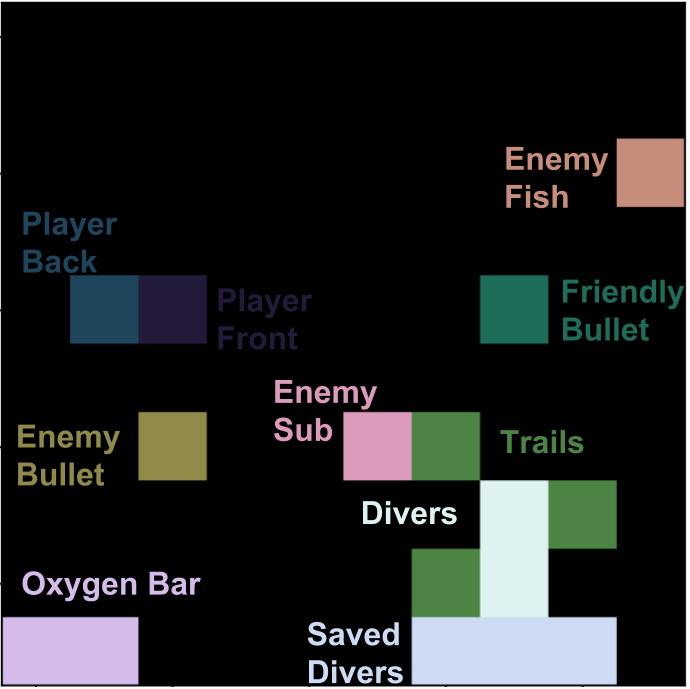
\includegraphics[width=0.19\textwidth]{annotated_seaquest.png} &
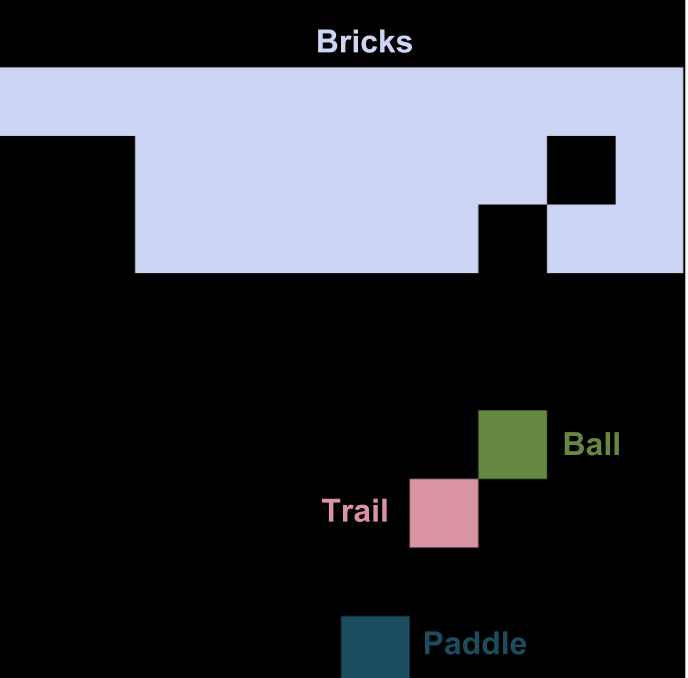
\includegraphics[width=0.19\textwidth]{annotated_breakout.png} &
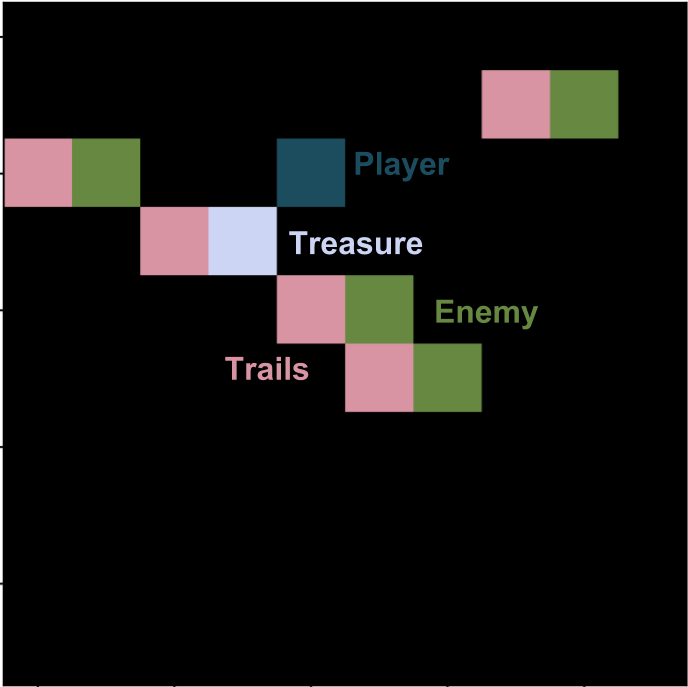
\includegraphics[width=0.19\textwidth]{annotated_asterix.png} &
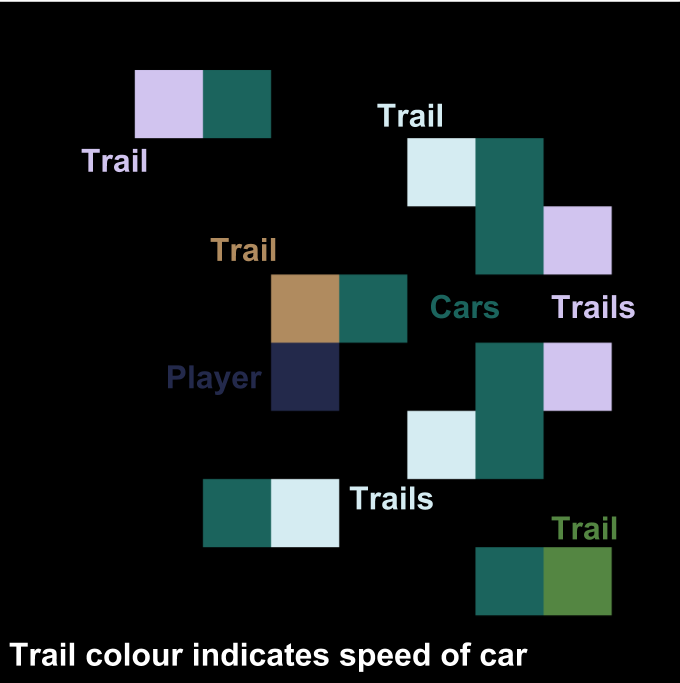
\includegraphics[width=0.19\textwidth]{annotated_freeway.png} &
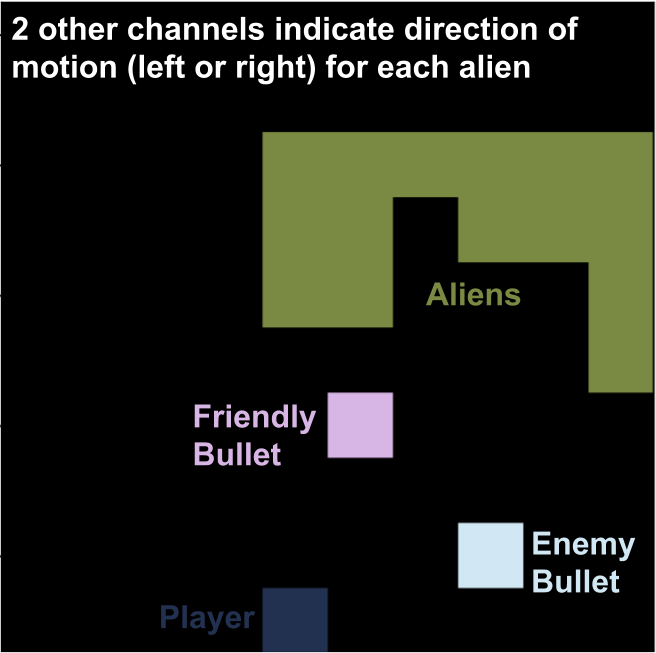
\includegraphics[width=0.19\textwidth]{annotated_space_invaders.png} \\
\emph{Seaquest} & \emph{Breakout} & \emph{Asterix} & \emph{Freeway} & \emph{Space Invaders}
\end{tabular}
\caption{Visualisation of each MinAtar environment. Colour indicates active channel at each spatial location, but
note that the representation provided by the environment consists of binary values for each channel and not RGB
values. Reproduced from \citet{young2019minatar}.}
\label{fig:minatar}
\end{figure*}

The arms were trained on four MinAtar games \citep{young2019minatar} (Fig.~\ref{fig:minatar}): Breakout, Asterix, Freeway and Space Invaders
(version~1, with the minimal action set). Each game is played on a $10\times10$ grid, and the agent observes a
$10\times10\times n$ binary state with one channel per game-specific object \citep{young2019minatar}: $n=4$ in Breakout and
Asterix, 7 in Freeway and 6 in Space Invaders. MinAtar's default settings were kept, including sticky actions with
probability 0.1 \citep{young2019minatar} and difficulty ramping in the games that support it. Seaquest was also run but
is excluded: in each of the four arms in which it was run, a greedy evaluation episode exceeded the 100,000-step limit, because
MinAtar never ends a Seaquest episode in which the submarine stays on the surface, where it starts. No run in the
four reported games was aborted. The trial therefore comprises $4\times5\times30=600$ runs.

\subsection{Agent and Shared Training Recipe}
Table~\ref{tab:settings} lists the training settings. All arms use the network of the MinAtar DQN
baseline \citep{young2019minatar}, whose 16 filters and 128 hidden units are a quarter of the corresponding layers of
DQN \citep{mnih2015human}; whether there are one or two hidden layers is sampled. Training uses
RMSProp \citep{tieleman2012rmsprop} with the MSE loss~\eqref{eq:loss}. MinAtar has no frame skipping, so a frame is
one environment step, and each run lasts $5\times10^{6}$ frames, as in the MinAtar baselines.

\begin{table}[t]
\caption{Training Settings}
\label{tab:settings}
\centering
\footnotesize
\begin{tabular}{@{}l>{\raggedright\arraybackslash}p{0.66\columnwidth}@{}}
\toprule
Setting & Value \\
\midrule
Network & convolution ($16$ filters, $3\times3$, stride 1), then 1 or 2 hidden layers of 128 units (ReLU) \\
Optimiser, loss & RMSProp (decay 0.99, $\epsilon=10^{-8}$, no momentum); MSE \\
Discount, exploration & $\gamma=0.99$; $\varepsilon$ from 1.0 to 0.1, linear over the sampled duration \\
Updates & one per step after 5,000 random transitions \\
Training length & $5\times10^{6}$ frames (no frame skipping) \\
Evaluation & every $5\times10^{4}$ frames; 10 greedy episodes with seeds 1000--1009 \\
\midrule
PER & proportional; $\alpha=0.6$; $\beta$ from 0.4 to 1 over training; $\epsilon=10^{-6}$ \\
$n$-step DQN & $n=3$; no off-policy correction \\
Averaged DQN & $K=10$ target networks, one stored at each target update \\
\bottomrule
\end{tabular}
\end{table}

The recipe is deliberately shared and is not the recipe of any one paper: DQN is usually trained with the Huber
loss \citep{obandoceron2021revisiting}, and \citet{schaul2016prioritized} lowered the step size for PER.
Changing one component under a fixed recipe is what isolates its effect, but it also means that the results concern
these components under this recipe.

The treatments were implemented as follows. PER stores priorities in a sum tree, draws each mini-batch by stratified
sampling over equal segments of the total priority, normalises the importance weights by the largest possible weight,
anneals $\beta$ linearly over the $5\times10^{6}$ frames and averages the weighted squared TD errors. $n$-step DQN
stores, for each transition, the discounted sum of the next three rewards and the state three steps later; at the
end of an episode, the remaining shorter returns are stored without a bootstrap. Averaged DQN stores a copy of the
target network at every target update and averages the last ten copies as in~\eqref{eq:avg}, or all of them while
fewer than ten exist.

\subsection{Evaluation and Primary Outcome}
Every $5\times10^{4}$ frames, the online network was evaluated greedily ($\varepsilon=0$) for 10 episodes, with the
same environment seeds (1000--1009) for every individual, arm and checkpoint. The mean return $G_i$ at checkpoint $i$
is one point on the evaluation curve, giving 100 points per run. An evaluation episode longer than $10^{5}$ steps
aborts the run without recording a score. The primary outcome is the trapezoidal area under the curve,
\begin{equation}
\mathrm{AUC}=\sum_{i=1}^{99}\frac{G_i+G_{i+1}}{2}\,\Delta x,\qquad \Delta x=5\times10^{4}\ \text{frames},
\end{equation}
reported in units of $10^{6}$ (return $\times$ frames). The AUC rewards both fast learning and a high final level:
divided by the $4.95\times10^{6}$ frames it spans, it is the average evaluation return over training.

\subsection{Statistical Analysis}\label{sec:stats}
The statistical unit is the individual. The ten evaluation episodes at a checkpoint and the 100 checkpoints of a run
all measure the same agent, so they are repeated measurements within one run rather than independent replicates;
treating them as separate observations would inflate the sample size and understate the uncertainty. Each run
therefore contributes one AUC. For each game and treatment, we form the 30 paired differences
$d_j=\mathrm{AUC}_j^{\mathrm{treatment}}-\mathrm{AUC}_j^{\mathrm{DQN}}$ and test whether their mean is zero with a
two-sided paired $t$-test. Because our conclusions are drawn across games, we treat all $4\times4=16$ comparisons as
one family and apply the Bonferroni correction \citep{dunn1961multiple}, $\alpha=0.05/16=0.003125$, with matching
simultaneous 99.69\% $t$-intervals. We report each effect as the mean difference as a percentage of the DQN mean, with
the standardised effect $d_z=\bar d/s_d$ \citep{lakens2013calculating} and the number of individuals for which the
treatment beat DQN. We report the $t$-test as primary and the Wilcoxon signed-rank test \citep{wilcoxon1945individual}
as a sensitivity analysis for every comparison, rather than choosing between them with a normality pre-test, which
alters the error rates of the test that follows \citep{rochon2012test}; Shapiro--Wilk \citep{shapiro1965analysis}
rejected normality of the differences at the 0.05 level for 6 of the 16 comparisons.

A percentage of the DQN mean divides the mean difference, and its interval, by the DQN mean as if that mean were
known exactly. Because the AUC is positive, no arm can be more than 100\% worse than DQN, yet the interval can extend
below $-100\%$ when the differences vary widely relative to the DQN mean: for $n$-step DQN in Asterix it is
[$-131.3\%$, $-28.8\%$]. We therefore also analyse the per-individual log ratios
$\log(\mathrm{AUC}_j^{\mathrm{treatment}}/\mathrm{AUC}_j^{\mathrm{DQN}})$: their back-transformed mean is the
geometric-mean ratio, which we report with the same 99.69\% $t$-interval and a one-sample $t$-test ($p_r$).

Two secondary endpoints address RQ2: the mean of the last ten evaluations (the final $5\times10^{5}$ frames) and the
final evaluation alone. The fraction of individuals for which a treatment beats DQN estimates the probability that it
does so on a randomly drawn configuration, a paired analogue of the probability of improvement of
\citet{agarwal2021deep}; we give 95\% Wilson intervals \citep{wilson1927probable}. To mimic smaller trials, we repeat
each significant comparison on every subset of $k\in\{3,5\}$ individuals and on $10^{5}$ random subsets of $k=10$, and
record how often a paired $t$-test at $\alpha=0.05$ detects the effect in the direction of the full trial. To mimic
separately tuned methods, we compare the best AUC of each arm over the 30 configurations with that of DQN, a comparison
that is biased upwards and only illustrative. Finally, as the six hyperparameters were sampled independently, we
regress log AUC on all six, as categorical factors, for each arm and game. The bands in the learning curves are
pointwise 95\% bootstrap intervals over individuals (2,000 resamples, \citealt{efron1979bootstrap}). All analyses
other than the Bonferroni-corrected paired $t$-tests on the AUC are exploratory.

\subsection{Implementation}\label{sec:implementation}
The agents were implemented in PyTorch \citep{paszke2019pytorch} (version 2.13) with the
Gymnasium \citep{towers2024gymnasium} interface to MinAtar (version 1.0.15) and trained on CPUs, with four threads
per job, on the MSL cluster at the University of the Witwatersrand. The code includes unit tests and analytic checks
of every arm's target and replay computations, which run before each cluster job. Among them, PER's sampling
probabilities and importance weights are checked against analytic values, $n$-step returns against an independent
episode-level reference, and $n$-step DQN with $n=1$ is checked to reproduce the network weights of DQN exactly through
the MinAtar training loop.

% =====================================================================================
\section{Results}\label{sec:results}

\begin{table*}[t]
\caption{Mean AUC ($10^{6}$, Standard Deviation in Parentheses) and Paired Comparisons with DQN ($n=30$ per Arm)}
\label{tab:main}
\centering
\footnotesize
\setlength{\tabcolsep}{4.5pt}
\input{\results/tab_main.tex}\\[3pt]
\parbox{\textwidth}{\scriptsize $\Delta$: mean paired difference as a percentage of the DQN mean. Ratio: geometric
mean of the per-individual ratio of the treatment's AUC to that of DQN, with its Bonferroni-adjusted 99.69\%
$t$-interval on the log scale. $d_z$: mean difference divided by the standard deviation of the differences. $p_t$,
$p_W$: two-sided paired $t$-test and Wilcoxon signed-rank $p$-values (primary analysis); $p_r$: one-sample $t$-test of
the log ratios. Bold values are at most $0.05/16$.}
\end{table*}

\begin{figure}[t]
\centering
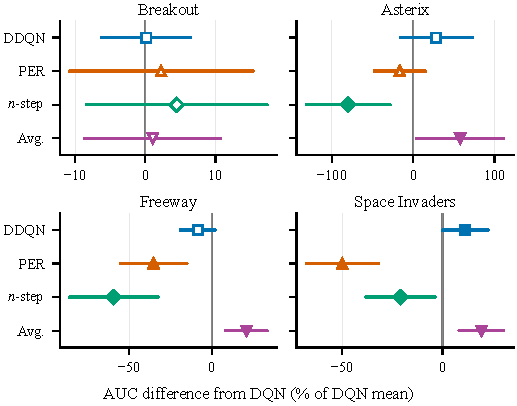
\includegraphics[width=\columnwidth]{paired_effects.pdf}
\caption{Geometric-mean AUC ratio of each treatment to DQN, on a log scale, with Bonferroni-adjusted 99.69\%
intervals. Filled markers: significant in the primary paired $t$-test ($p_t\le0.05/16$). The horizontal scales differ
between games. DDQN: Double DQN; Avg.: Averaged DQN.}
\label{fig:effects}
\end{figure}

\begin{figure*}[t]
\centering
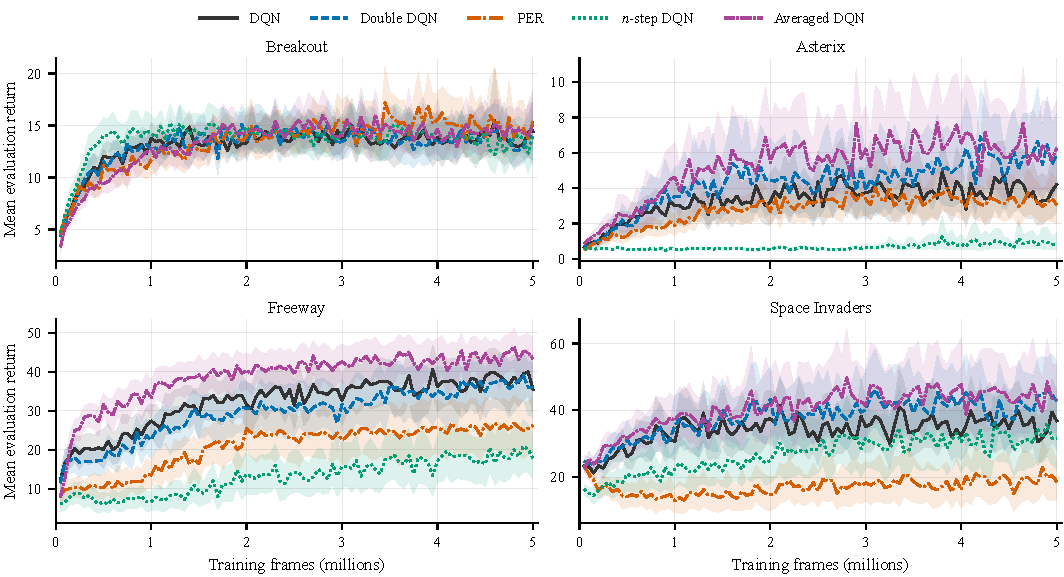
\includegraphics[width=\textwidth]{learning_curves.pdf}
\caption{Mean greedy evaluation return during training ($n=30$ individuals per arm). Shaded bands are pointwise
95\% bootstrap intervals over individuals; the curves are not smoothed.}
\label{fig:curves}
\end{figure*}

\subsection{Primary Outcome}
Table~\ref{tab:main} and Fig.~\ref{fig:effects} report the 16 comparisons, nine of which are significant at the
family-wide threshold. Averaged DQN had a higher AUC than DQN in Asterix ($+57.5\%$), Freeway ($+20.9\%$) and Space
Invaders ($+19.5\%$), and beat DQN on 25, 24 and 26 of the 30 individuals. Double DQN was better only in Space
Invaders ($+11.4\%$, 21 of 30 individuals); its differences in Asterix ($+28.2\%$, $p_t=0.048$) and Freeway
($-8.5\%$, $p_t=0.014$) were not significant. PER was worse in Freeway ($-35.3\%$) and Space Invaders ($-50.0\%$),
beating DQN on only 3 and 1 individuals. $n$-step DQN was worse in Asterix ($-80.0\%$), Freeway ($-59.4\%$) and Space
Invaders ($-21.0\%$), with 2, 0 and 6 wins. The significant effects have $|d_z|$ between 0.59 and 1.64.
Holm's step-down procedure \citep{holm1979simple}, which is uniformly at least as powerful as the Bonferroni correction,
rejects the same nine hypotheses: the tenth-smallest $p$-value, 0.014, exceeds $0.05/7$.

On the ratio scale, seven of the nine findings remain significant at the family-wide threshold
(Table~\ref{tab:main}, Fig.~\ref{fig:effects}). The two exceptions are gains. Averaged DQN in Asterix has a
geometric-mean ratio of 1.38 $[0.89, 2.12]$ ($p_r=0.024$): it beat DQN on 25 individuals, but on two others it reached
only 0.10 and 0.28 of the AUC of DQN, and these dominate on the log scale; a Wilcoxon test on the log ratios still
rejects ($p=0.0016$). Double DQN in Space Invaders has a ratio of 1.10 $[0.97, 1.26]$ ($p_r=0.023$). The log ratios
were not closer to normal than the differences: Shapiro--Wilk rejected normality for 9 of the 16 comparisons.

In Breakout no treatment differed significantly from DQN. The ratios lie between 1.00 and 1.03, but their intervals
extend from 0.89 to 1.18, so the data do not show that the extensions are equivalent to DQN there either.

\subsection{Learning Dynamics}
The learning curves (Fig.~\ref{fig:curves}) show how these differences arise. In Breakout the curves rise quickly
and then overlap for the rest of training, ending between 13.2 and 14.8 (mean of the last ten evaluations); $n$-step
DQN learnt fastest early on, with a mean return of 14.0 against 12.0 for DQN at $5\times10^{5}$ frames. In Asterix,
$n$-step DQN barely improved: its mean curve never exceeded 1.24, whereas DQN ended at 3.8. In Freeway, Averaged DQN
led from early in training (31.6 against 20.1 for DQN at $5\times10^{5}$ frames) and ended highest (44.1 against
38.4). In Space Invaders, PER started level with DQN (23.6 against 23.5 at the first evaluation), fell to 13.0 by
$10^{6}$ frames and ended at about half the level of DQN (19.1 against 35.9).

\subsection{Variation Across Configurations}\label{sec:variation}
Performance varied widely between configurations (Fig.~\ref{fig:dist}). For DQN, the standard deviation of
the AUC across individuals ranged from 26\% (Breakout) to 84\% (Asterix) of its mean. The paired design removes the
main effect of the configuration from the comparisons; the interaction between configuration and treatment remains
in the variance of the differences. Several of the distributions are skewed or have more than one mode. The most
extreme are those of $n$-step DQN: in Asterix, 29 of its 30 individuals had an AUC of at most 5, and in Freeway its
seven individuals at the lowest learning rate all had an AUC between 8.2 and 28.0, against 144.8 to 231.9 for DQN at
that rate.

\begin{figure}[t]
\centering
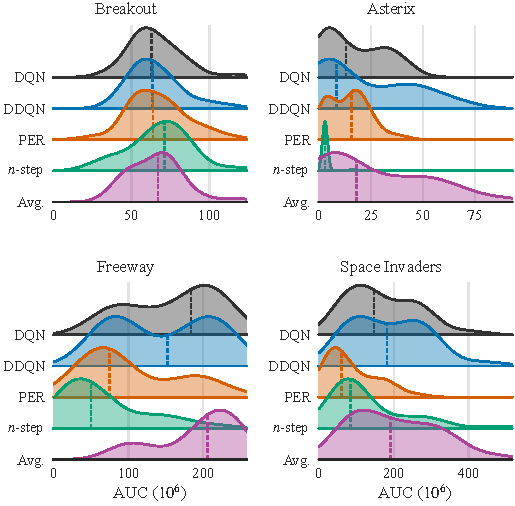
\includegraphics[width=\columnwidth]{auc_density.pdf}
\caption{Distribution of the AUC over the 30 individuals of each arm, in the style of \citet{pretorius2020dropout}:
Gaussian kernel density estimates (Scott's bandwidth, clipped at zero), each scaled to its own peak height.
Dashed lines mark the medians. DDQN: Double DQN; Avg.: Averaged DQN.}
\label{fig:dist}
\end{figure}

\begin{figure}[t]
\centering
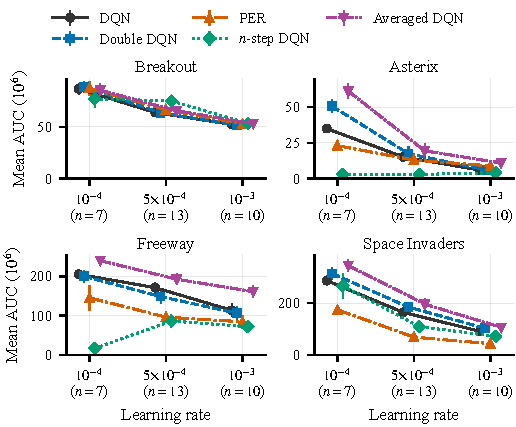
\includegraphics[width=\columnwidth]{learning_rate.pdf}
\caption{Mean AUC by sampled learning rate, with $\pm1$ standard error over the $n$ individuals at each rate. The
subgroups also differ in their other hyperparameters, so the comparison is descriptive;
Table~\ref{tab:regression} adjusts for them.}
\label{fig:lr}
\end{figure}

Much of this variation was associated with the learning rate (Fig.~\ref{fig:lr}). The mean AUC of DQN at a learning rate
of $10^{-4}$ was 1.7 to 5.9 times its mean at $10^{-3}$ (Breakout 86.5 against 52.2, Asterix 35.1 against 6.0,
Freeway 205.4 against 113.2, Space Invaders 287.9 against 90.8). Because these subgroups also differ in their other
hyperparameters, we regressed log AUC on all six sampled factors (Table~\ref{tab:regression},
Appendix~\ref{app:regression}). Adjusted for the other
five, raising the learning rate from $10^{-4}$ to $10^{-3}$ multiplied the AUC of DQN by 0.21 (Asterix) to 0.57
(Freeway), and the learning rate explained 58\% to 93\% of the variance in log AUC that the other factors left
unexplained (partial $R^2$). On this common log scale, the adjusted learning-rate effect on DQN was larger than the
geometric-mean treatment effect in 15 of the 16 comparisons; the exception was $n$-step DQN in Freeway. The lowest
learning rate gave the highest mean AUC for every arm in every game except $n$-step DQN in Asterix and Freeway.

The two $n$-step deficits responded differently to the learning rate. In Asterix, $n$-step DQN barely learnt at any
rate: its mean AUC was 3.0, 2.9 and 4.2 from the lowest rate to the highest, and its ratio of mean AUC to that of DQN rose from 0.09 to
0.70 only because DQN did worse at higher rates. In Freeway, by contrast, $n$-step DQN failed at $10^{-4}$, the rate at
which every other arm did best: its mean AUC there was 16.1, against 205.4 for DQN, whereas at the two larger rates it
reached 86.1 and 71.4 (ratios of means to DQN of 0.50 and 0.63). Adjusted for the other factors, its AUC at $10^{-3}$ was 4.12
$[2.31, 7.34]$ times that at $10^{-4}$, whereas the corresponding factor was below one for DQN, Double DQN and
Averaged DQN. PER stayed below DQN at every learning rate in Freeway and Space Invaders, with ratios of means to DQN between 0.41
and 0.74 and no consistent trend; at $10^{-4}$ the ratios were 0.71 and 0.61.

The gain of Averaged DQN did not shrink consistently at longer target-update periods: at periods of 500, 1000 and
2000 steps (8, 11 and 11 individuals), its geometric-mean ratio to DQN was 1.23, 1.25 and 1.27 in Freeway, 0.85,
1.78 and 1.51 in Asterix and 1.21, 1.26 and 1.08 in Space Invaders. In the regression, a period of 2000 rather than
500 steps changed the AUC of DQN itself by a factor of 0.83 to 1.12.

\subsection{Robustness}
The nine findings survive several checks. With a Bonferroni correction within each game instead
($\alpha=0.05/4=0.0125$), the same nine comparisons are significant. The Wilcoxon test confirms eight of them at the
family-wide threshold; the exception is Double DQN in Space Invaders ($p_W=0.012$), whose interval also only just
excludes zero ($[+0.1\%, +22.6\%]$), so this finding rests on the $t$-test alone.

The secondary endpoints (Table~\ref{tab:robust}) agree in direction with all nine findings, but they are noisier.
With the mean of the last ten evaluations, five of the nine remain significant at the family-wide threshold; with the
final evaluation alone, only three do. No comparison that was not significant on the AUC became significant on
either secondary endpoint. The single-checkpoint endpoints therefore have less power than the AUC; they do not point
to different conclusions.

\subsection{Reliability of Smaller Evaluations}\label{sec:reliability}

\begin{table}[t]
\caption{Reliability of Smaller Evaluations}
\label{tab:reliability}
\centering
\footnotesize
\setlength{\tabcolsep}{3.5pt}
\input{\results/tab_reliability.tex}\\[3pt]
\parbox{\columnwidth}{\scriptsize PoI: fraction of individuals for which the treatment's AUC exceeds that of DQN,
with 95\% Wilson interval. Best of 30: best AUC of the arm over the 30 configurations relative to the best of DQN.
Detected: percentage of subsets of $k$ individuals in which a paired $t$-test at $\alpha=0.05$ is significant in the
direction of the full trial (all subsets for $k=3,5$; $10^{5}$ random subsets for $k=10$), shown for the nine
significant comparisons.}
\end{table}

Table~\ref{tab:reliability} shows how smaller or more typical evaluations would have fared. The paired probability of
improvement of Averaged DQN was 0.83, 0.80 and 0.87 in Asterix, Freeway and Space Invaders, so a comparison on one
configuration drawn at random would have favoured DQN with a probability of 0.13 to 0.20. Trials of a few
configurations usually got the direction of a finding right: the mean difference had the sign of the full trial in
84\% to 100\% of the subsets of three individuals and 92\% to 100\% of those of five. They seldom reached
significance, however: a $t$-test detected the effects in 6\% to 30\% of the subsets of three, 9\% to 79\% of those of
five and 37\% to 100\% of those of ten, and detected the two weakest findings, Double DQN in Space Invaders and
Averaged DQN in Asterix, in fewer than half of the subsets of ten. Significance in the wrong direction occurred in at
most 0.4\% of subsets. Comparing the best configuration of each arm with that of DQN, as a study that tunes each
method separately would, reversed two findings: $n$-step DQN was $24.7\%$ better than DQN in Space Invaders and PER
$2.0\%$ better in Freeway.

% =====================================================================================
\section{Discussion}\label{sec:discussion}

\subsection{RQ1: Which Extensions Help?}
Averaged DQN was the only extension that improved on DQN in more than one game, on at least 24 of 30 individuals in
each of three games, and the Wilcoxon test confirmed all three; on the ratio scale its gain in Asterix was not
significant. It was designed to reduce the variance of the target \citep{anschel2017averaged}, which we did not
measure. Averaging ten target networks also makes the target depend on older parameters; if that were the cause, the
gain should shrink at long target-update periods and long periods should help DQN, but neither happened consistently
(Section~\ref{sec:variation}).

Double DQN helped little. Its one significant result, in Space Invaders, was the weakest of the nine findings: neither
the Wilcoxon test nor the ratio scale confirmed it, and its other estimates had mixed signs. We did not measure
overestimation, so we cannot tell whether it was small under this recipe or whether reducing it did not raise the AUC.

PER and $n$-step returns were harmful, unlike in the Rainbow ablation on Atari \citep{hessel2018rainbow} and, for
$n$-step returns, the MinAtar study of \citet{obandoceron2021revisiting}. Is this the recipe or an implementation
error? The analytic checks of every arm (Section~\ref{sec:implementation}) make a gross error unlikely, but they cannot exclude an interaction between our implementation and the recipe. Without a
positive control, such as DQN against PER and $n$-step DQN under the recipe of Obando-Ceron and Castro, the
explanations below are hypotheses.

\citet{schaul2016prioritized} reduced the step size for PER, and Obando-Ceron and Castro used Adam with one update
every four steps, whereas we used RMSProp with the MSE loss and one update per step; with RMSProp, they found that the
Huber loss tended to work better than the MSE on Atari, although Adam with the MSE loss was their best combination. A step size too large for PER should matter least at the
lowest learning rate, yet PER remained 29\% and 39\% below DQN at $10^{-4}$ in Freeway and Space Invaders, so the step
size alone does not explain its deficit. Because non-uniform sampling has the same expected gradient as a different
loss under uniform sampling \citep{fujimoto2020equivalence}, PER with the MSE may weight large errors more heavily than
intended; recording the importance weights and TD errors during training would allow this to be examined. PER's own
settings were also fixed rather than sampled: $\alpha$ and $\beta_0$ were chosen by \citet{schaul2016prioritized} with
Double DQN on Atari, and $\epsilon=10^{-6}$ is our choice. Other values could change the effect of PER, and the trial
cannot show how much, because they were not varied.

The two $n$-step deficits differ in kind (Section~\ref{sec:variation}). In Asterix, $n$-step DQN barely learnt at any
learning rate. In Freeway, it failed at the rate at which every other arm did best and partly recovered at larger
rates, an interaction that a study tuning each method separately would not see. We found no consistent association
with the replay buffer capacity, the factor that \citet{fedus2020revisiting} identified for $n$-step returns, but the
subgroups are small.

\subsection{RQ2: How Reliable Are Smaller Evaluations?}
Evaluating whole learning curves over a population of configurations exposes how unreliable smaller or more typical
evaluations are (Section~\ref{sec:reliability}). The single-checkpoint endpoints
differed from the AUC in power, not in conclusions: they agreed in direction with all nine findings but detected only
three or five. Small trials usually pointed the right way but seldom reached significance, so the absence of a
significant effect in a small evaluation says little. Comparing the best configuration of each method, as separately
tuned studies effectively do, reversed two findings, because the effects depend on the configuration.

The paired design makes the effects detectable despite this dependence: the significant effects have $|d_z|$ between
0.59 and 1.64, whereas the spread of the AUC between individuals is often as large as the differences between arms
(Fig.~\ref{fig:dist}).

Isolated under a shared recipe, the effects only partly matched those reported in the literature: the benefits
reported for PER and $n$-step returns did not appear, whereas those of Averaged DQN did.

% =====================================================================================
\section{Limitations}\label{sec:limitations}
Each configuration was trained with one seed, so within an individual the effects of the configuration and the seed
cannot be separated; both are shared across arms, so the comparisons remain paired. The results hold for one shared
recipe with treatment settings fixed at published values or, for PER's $\epsilon$, our own choice; tuning each arm separately could change them, and without a
positive control under another recipe an interaction between our implementation and the recipe cannot be fully
excluded. The grid of learning rates does not bracket the optimum: the lowest rate was best for almost every arm, so
the treatment effects are conditional on a population in which 23 of the 30 configurations probably use too large a
learning rate. The trial covers four MinAtar games and $5\times10^{6}$ frames. Seaquest was lost to a protocol choice:
the evaluation aborted a run whose greedy episode exceeded $10^{5}$ steps instead of capping the episode, which would
have kept the game in the trial. The subgroup analyses are descriptive, and all analyses beyond the primary
comparisons are exploratory (Section~\ref{sec:stats}).

% =====================================================================================
\section{Conclusion}
In a paired randomised control trial of four DQN extensions over 30 sampled configurations and four MinAtar games,
only Averaged DQN improved on DQN in more than one game. Double DQN helped only slightly and not robustly, and
prioritised replay and multi-step returns were harmful under the shared recipe, contrary to earlier component studies.
The learning rate changed performance by as much as the largest treatment effects, small evaluations detected fewer
of the findings, and comparing the best configuration of each method reversed two of them. Future work should run a
positive control under the recipe of \citet{obandoceron2021revisiting}, add learning rates below $10^{-4}$, the lowest rate tested and the best for almost every arm, add
seeds per configuration, and evaluate Seaquest with a capped protocol.

\section*{Acknowledgement}
I express my sincere gratitude to my supervisors, Steven James and Benjamin Rosman,
for their invaluable guidance, patience, and continuous support throughout the formulation of this research report.

\bibliographystyle{plainnat}
\bibliography{refs}

\appendices
\section{Additional Results}\label{app:results}
Table~\ref{tab:robust} gives the paired comparisons on the two secondary endpoints.

\begin{table}[h]
\caption{Secondary Endpoints: Paired Comparisons with DQN}
\label{tab:robust}
\centering
\footnotesize
\setlength{\tabcolsep}{4pt}
\input{\results/tab_robustness.tex}\\[3pt]
\parbox{\columnwidth}{\scriptsize $\Delta$ and $p_t$ as in Table~\ref{tab:main}; bold: $p_t\le0.05/16$. DDQN: Double DQN; Avg.: Averaged DQN. These
endpoints are exploratory.}
\end{table}

\section{Learning-Rate Regression}\label{app:regression}
Table~\ref{tab:regression} gives, for every arm and game, the ordinary least-squares regression of log AUC on the six
sampled hyperparameters, each coded as a categorical factor with its first value as the reference (11 coefficients,
19 residual degrees of freedom). The learning-rate ratio is the back-transformed coefficient of $10^{-3}$ relative to
$10^{-4}$; the partial $R^2$ is the share of the variance left by the other five factors that the learning rate
explains.

\begin{table}[h]
\caption{Adjusted Learning-Rate Effect on Log AUC}
\label{tab:regression}
\centering
\footnotesize
\input{\results/tab_regression.tex}\\[3pt]
\parbox{\columnwidth}{\scriptsize LR ratio: multiplicative change in AUC from a learning rate of $10^{-4}$ to
$10^{-3}$, adjusted for the other five hyperparameters, with 95\% $t$-interval. Partial $R^2$: of the learning rate
given the other factors. $R^2$: of the full model.}
\end{table}

\end{document}
